\usepackage{amsthm}

\newtheorem{theorem}{Theorem}[chapter]
\newtheorem{lemma}           [theorem] {Lemma}   
\newtheorem{folg}           [theorem] {Folgerung}   

\newtheorem{frage}       [theorem] {Frage}   
\newtheorem{question}       [theorem] {Question}   
\newtheorem{aufgabe}       [theorem] {Aufgabe}   
\newtheorem{exercise}       [theorem] {Exercise}  

\newtheorem{proposition}     [theorem] {Proposition}  
\newtheorem{satz}     [theorem] {Satz}  
\newtheorem{fact}{Fact}
\newtheorem{definition}      [theorem] {Definition} 

\theoremstyle{definition} 
\newtheorem{bemerkung}     [theorem] {Bemerkung}  
\newtheorem{beispiel}       [theorem] {Beispiel}  
\newtheorem{example}       [theorem] {Example}  
\newtheorem*{example*} {Example}  
\newtheorem{notation}       [theorem] {Notation}  
\newtheorem*{Faust}[theorem]{Rule of Thumb}
\newtheorem*{Boxx}[theorem]{Concept}

%\section{Logarithm}
We will now define the logarithm as the inverse function of the exponential function. As we have seen, the exponential function is bijective as a~map from $\mathbb{R}$ to $(0,\infty)$. This justifies the following definition.
\begin{Definition}{}
 The \emph{(natural) logarithm} $\log:(0,\infty)\to\mathbb{R}$ is defined as the inverse function of $\exp:\mathbb{R}\to(0,\infty)$, i.e., for all $x\in\mathbb{R}$ holds $\log(\exp(x))=x$ and for all $y \in (0,\infty)$ holds $\exp(\log(y)) = y$.
\end{Definition}
In many books, the above defined function is also denoted by {\em logarithmus naturalis} $\ln$. Before we collect some properties, a~general result about continuity of inverse functions is presented.


\begin{Theorem}{Continuity of the inverse function}\label{thm:invcont}
Let $I,J\subset\mathbb{R}$ be open intervals and let $f:I\to J$ be a~continuous, bijective and strictly monotonically increasing (or decreasing) function. 
Then the inverse function $f^{-1}:J\to I$ is continuous and strictly monotonically increasing (resp.\ decreasing).
\end{Theorem}
{\em Proof:} 
First we show strict monotonic increase. Let $y_1,y_2\in J$ with $y_1< y_2$. Then
  \[f(f^{-1}(y_1))=y_1 < y_2 = f(f^{-1}(y_2))\]
  shows that, since $f$ is strictly monotonically increasing, $f^{-1}(y_1)\geq f^{-1}(y_2)$ cannot hold, so that $f^{-1}(y_1) < f^{-1}(y_2)$.
  But this means that $f^{-1}$ is strictly monotonically increasing.

Now we show continuity. 
Let $\eps>0$ and $y_0\in J=f(I)$. Set $x_0:=f^{-1}(y_0)\in I$. Since $I$ is an open interval, there is  
an $\eps'>0$ with $\eps'<\eps$ such that $[x_0-\eps',x_0+\eps']\subset I$. 
Since $f$ is strictly monotonically increasing, $$\delta:=\min\{f(x_0+\eps')-y_0,y_0-f(x_0-\eps')\}>0.$$
Then for $y\in J$ with $|y-y_0|<\delta$ holds $f(x_0-\eps')< y< f(x_0+\eps')$ and the intermediate value theorem 
yields $$x:=f^{-1}(y) \in [x_0-\eps',x_0+\eps'] \subset ~ (x_0-\eps,x_0+\eps) ~ = ~ (f^{-1}(y_0)-\eps,f^{-1}(y_0)+\eps)\ ,$$
i.e. $|f^{-1}(y)-f^{-1}(y_0)|<\eps$. By the $\eps$-$\delta$  criterion this means that $f^{-1}$ is continuous in $y_0$. 
\hfill$\Box$
\\ \\
We want to remark that Theorem \ref{thm:invcont} also holds for intervals $I$ and $J$ which are not open. 
In this case the proof of continuity of $f^{-1}$ in $y_0\in J$ has to be slightly adapted for boundary points $x_0:=f^{-1}(y_0)$. 
This was dropped for simplicity reasons. 
  

\begin{Theorem}{Properties of the Logarithm}
 \begin{enumerate}[(i)]
\item For all $x,y\in~(0,\infty)$ holds $\log(x\cdot y)=\log(x)+\log(y)$.
\item $\log:~(0,\infty)~\to~\mathbb{R}$ is strictly monotonically increasing.
\item $\log:~(0,\infty)~\to~\mathbb{R}$ is continuous.
\end{enumerate}
\end{Theorem}
\white{6cm}{
{\em Proof:}
 \begin{enumerate}[(i)]
\item Define $x_1=\log(x)$ and $y_1=\log(y)$. Then, using $x=\exp(x_1)$ and $y=\exp(y_1)$, we obtain
\[\log(x\cdot y)=\log(\exp(x_1)\cdot \exp(y_1))=\log(\exp(x_1+y_1))=x_1+y_1=\log(x)+\log(y).\]
\end{enumerate}
(ii) and (iii) follow from Theorem~\ref{thm:invcont}.\hfill$\Box$
}

% \begin{figure}[h!]
% \begin{center}
% 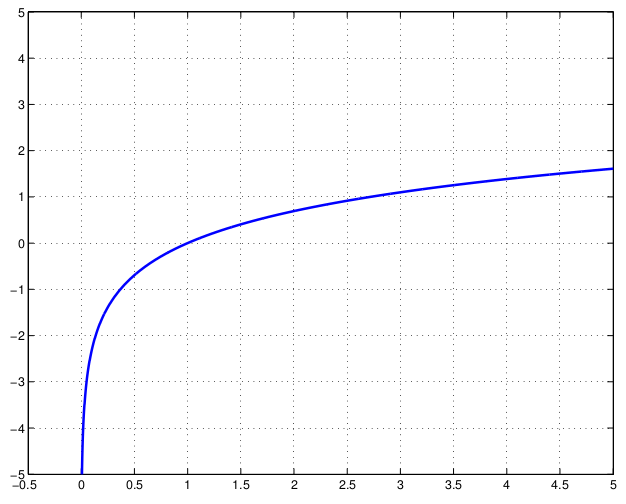
\includegraphics[width=0.81\textwidth,angle=0]{pics/log.eps}
% \caption{Graph of the logarithm}\label{fig:log}
% \end{center}
% \end{figure}

% \begin{Remark}{}
% Without further ado we introduce the logarithm for complex numbers $z=r\exp(i\varphi)$ in polar coordinates with $r>0$ and $\varphi\in [0,2\pi)$  
% by $$\log(r\exp(i\varphi))=\log(r)+\log(\exp(i\varphi))=\log(r)+i\varphi \ .$$
% However, formally this is a quite delicate issue and not treated in this lecture in much detail. 
% For further information on complex logarithms we refer to books on {\em Complex Analysis} (German: {\em Funktionentheorie}).
% \end{Remark}
% By means of the exponential function, the {\em general power} $a^x$ (for $a>0$, $x\in\mathbb{C}$) can be defined as follows:
% \[a^x:=\exp(\log(a)\cdot x).\]
% This definition indeed makes sense as $a^0=\exp(\log(a)\cdot 0)=1$, $a^1=\exp(\log(a)\cdot~1)=a$ and (for $n\in\mathbb{N}$)
% \[a^n=\exp(\underbrace{\log(a)+\ldots+\log(a)}_{n-\text{times}})=\exp(\log(a))^n.\]
% It can further be seen that this definition implies $a^{\frac1n}=\sqrt[n]{a}$. The definition of the general power also justifies the notion $\exp(x)=e^x$.\\
% A~remaining question is how to solve the equation
% \[a^x=y\]
% for given $a>0$, $y\in\mathbb{R}$ and unknown $x\in\mathbb{R}$. Using the definition of the general power, this equation becomes
% \[\exp(\log(a)\cdot x)=y.\]
% Performing the logarithm on both sides of this equation, we obtain 
% $\log(a)\cdot x=\log(y)$ and thus
% \[x=\frac{\log(y)}{\log(a)}.\]
% In some literature, this expression is known as the {\em logarithm of $y$ to the basis $a$} and abbreviated by
% \[\log_a(y):=\frac{\log(y)}{\log(a)}.\]
% By definition, we have $\log(x)=\log_e(x)$.
% 
% \begin{Remark}{The pocket calculator and high school maths}
% In most of high school literature the logarithm (as we have defined it) is called {\em natural logarithm} and is abreviated by $\ln$. 
% However, in mathematical literature the symbol $\log$ is also commonly used for the inverse function of $\exp$.\\
% Furthermore, note that for many pocket calculators, the button \texttt{log} stands for $\log_{10}$, the so-called {\em decimal logarithm}, 
% whereas pushing the button \texttt{ln} gives the logarithm.\\
% Note that the decimal logarithm is given by
% \[\log_{10}(x)=\frac{\log(x)}{\log(10)}.\]
% \end{Remark}


%  \section{Hyperbolic and Trigonometric Functions}
%  \subsection{Hyperbolic Functions}
%  \begin{Definition}{Hyperbolic Sine and Hyperbolic Cosine}
%  The \emph{hyperbolic sine (sinus hyperbolicus)} and \emph{hyperbolic cosine (cosinus hyperbolicus)} $\sinh:\mathbb{C}\to\mathbb{C}$ and $\cosh:\mathbb{C}\to\mathbb{C}$ are defined as
%  \[\sinh(x)=\frac12\left(\exp(x)-\exp(-x)\right),\qquad\cosh(x)=\frac12\left(\exp(x)+\exp(-x)\right).\]
%  \end{Definition}
%  \begin{figure}[H]
%  \begin{center}
%  \includegraphics[width=0.81\textwidth,angle=0]{pics/hyperb.eps}
%  \caption{Graph of the hyperbolic functions}\label{fig:hyp}
%  \end{center}
%  \end{figure}
%  \begin{Theorem}{Properties of the Hyperbolic Functions}\label{th:hyperbolicfunc}
%  \begin{enumerate}[(i)]
%  \item For all $x\in\mathbb{C}$ holds $\sinh(\overline{x})=\overline{\sinh(x)}$,  $\cosh(\overline{x})=\overline{\cosh(x)}$.
%  \item $\sinh$ and $\cosh$ are continuous.
%  \item For all $x\in\mathbb{C}$ holds $\cosh^2(x)-\sinh^2(x)=1$.
%  \item For all $x\in\mathbb{C}$ holds
%  \[\cosh(x)=\sum_{k=0}^\infty\frac{x^{2k}}{(2k)!},\qquad
%  \sinh(x)=\sum_{k=0}^\infty\frac{x^{2k+1}}{(2k+1)!}.\]
%  \item $\sinh:\mathbb{R}\to\mathbb{R}$ is strictly monotonically increasing.
%  \item $\cosh:\mathbb{R}\to\mathbb{R}$ is strictly monotonically increasing on $[0,\infty)$ and strictly monotonically decreasing on $(-\infty,0]$.
%  \end{enumerate}
%  \end{Theorem}
%  \begin{proof}
%  (i) and (ii) follow from Theorem~\ref{thm:expprop}.\\
%  (iii):
%  \begin{align*}
%  \cosh^{2}(x)-\sinh^{2}(x)&=\frac{1}{4}\left ((e^{x})^{2}+2e^{x}e^{-x}+(e^{-x})^{2}-(e^{x})^{2}+2e^{x}e^{-x}-(e^{-x})^{2} \right)\\
%  &=\frac{1}{4}\cdot4e^{x}e^{-x}=1.
%  \end{align*}
%  (iv): Using the series representation for $\exp$ we have
%  \begin{align*}
%  \sinh(x)&=\frac{1}{2}(e^{x}-e^{-x}) = \frac{1}{2}\left(\sum_{k=0}^{\infty}\frac{x^{k}}{k!}-\sum_{k=0}^{\infty}\frac{(-x)^{k}}{k!}\right)\\
%  &=\frac{1}{2}\left(\sum_{k=0}^{\infty}\frac{x^{k}}{k!}-\sum_{k=0}^{\infty}(-1)^{k}\frac{x^{k}}{k!}\right)\\
%  &=\frac{1}{2}\left(2\sum_{k=1,3,5,\ldots}\frac{x^{k}}{k!}\right) = \sum_{k=0}^{\infty}\frac{x^{2k+1}}{(2k+1)!}.
%  \end{align*}
%  The series representation for $\cosh$ can be derived analogously.\\
%  (v): Let $x\in\mathbb{R}$ and $a>0$. Then $e^{a}>1$, $0<e^{-a}<1$ and
%  \begin{align*}
%  \sinh(x+a) = {\textstyle\frac12} (e^{x+a}-e^{-(x+a)})={\textstyle\frac12}(e^a e^{x}-e^{-a}e^{-x})>{\textstyle\frac12}(e^{x}-e^{-x})=\sinh(x).
%  \end{align*}
%  (vi): First of all it holds for $x\in\mathbb{R}$
%  $$
%  \cosh(-x)=\frac{1}{2}(e^{-x}+e^{x})=\frac{1}{2}(e^{x}+e^{-x})=\cosh(x).
%  $$
%  Now let $x\geq 0$. From (iii) we have $\cosh^{2}(x)=1+\sinh^{2}(x)$ and since  $\cosh(x)\geq 1$ and $\sinh(x)\geq 0$ for $x\geq 0$ it follows directly from (v) that $\cosh$ is strictly increasing on $[0,\infty[$.\\
%  Now let $x\leq 0$. Since $\cosh(-x)=\cosh(x)$ it follows from the first part that $\cosh$ is strictly decreasing on $[-\infty,0)$.
%  \end{proof}
%  
%  
%  \begin{Remark}{}
%  The definition of the hyperbolic functions imply that $\sinh(-x)=-\sinh(x)$ (resp.\ $\cosh(-x)=\cosh(x)$). 
%  A~function with this property is called {\em odd} (resp.\ even).\\
%  The monotonicity property of $\cosh$ together with the fact that $\cosh(0)=1$ imply that $\cosh$ does not have any real zeros. 
%  The hyperbolic sine function has only one zero at the origin.
%  \end{Remark}
%  
%  \begin{Remark}{}
%  Why are these functions called {\em hyperbolic functions}?
%  \begin{figure}[H]
%  \begin{center}
%  \begin{psfrags}
%  %\psfrag{s}{\small$(\cosh(t),\sinh(t))$}
%  \centering
%  \includegraphics[width=0.81\textwidth,angle=0]{pics/hyperbola.eps}%{sinhcoshcurve.eps}
%  \end{psfrags}
%  \end{center}
%  \caption{Hyperbola}
%  \label{hyperbola}
%  \end{figure}
%  Since $\cosh^2(x)-\sinh^2(x)=1$, the curve 
%  $${\color{red} \{(-\cosh(t),\sinh(t)) ~|~t\in\mathbb{R}\}} \cup {\color{blue} \{(\cosh(t),\sinh(t)) ~|~t\in\mathbb{R}\}}$$ describes a~hyperbola 
%  see Figure \ref{hyperbola}.
%  (In analogy the curve $\{ (\cos(t),\sin(t))~|~t\in\mathbb{R}\}$ describes the unit circle.)
%  \\
%  \end{Remark}
%  
%  \begin{Definition}{Hyperbolic Tangent}
%  The \emph{hyperbolic tangent (tangens hyperbolicus)} $\tanh:\{x\in\mathbb{C}\,:\,\cosh(x)\neq0\}\to\mathbb{C}$ is defined as
%  \[\tanh(x)=\frac{\sinh(x)}{\cosh(x)} = \frac{e^{x}-e^{-x}}{e^{x}+e^{-x}}.\]
%  \end{Definition}
%  \begin{figure}[H]
%  \begin{center}\includegraphics[width=0.81\textwidth,angle=0]{pics/tanh.eps}
%  \caption{Graph of the hyperbolic tangent}\label{fig:tanh}
%  \end{center}
%  \end{figure}
%  \begin{Remark}{}
%  Since $\sinh$ and $\cosh$ map real numbers to real numbers and, moreover, $\cosh$ has no zero in $\mathbb{R}$, 
%  the hyperbolic tangent is defined on the whole real axis. Furthermore, it can be seen that $\tanh$ is continuous, strictly monotonically increasing and
%  \[\lim_{x\to\infty}\tanh(x)=1,\quad \lim_{x\to-\infty}\tanh(x)=-1.\]
%  \end{Remark}
%  
%  
%  
%  
%  
%  %  \subsection{Area Functions}
%  %  
%  %  We already know that $\sinh:\mathbb{R}\to\mathbb{R}$, $\cosh:[0,\infty)\to[1,\infty)$, $\tanh:\mathbb{R}\to\;\:(\!-\!1,1)$ are strictly monotonically increasing.
%  %  They possess inverse functions defined on $\mathbb{R}$ (resp.\ $[1,\infty)$, $(-1,1)$).
%  %  
%  %  \begin{Definition}{Area Functions}
%  %  \begin{enumerate}[(i)]
%  %  \item The \emph{area hyperbolic sine} or the \emph{area sinus hyperbolicus} 
%  %  $\arsinh:\:\mathbb{R}\to\mathbb{R}$ is defined as the inverse function of $\sinh$.
%  %  \item The \emph{area hyperbolic cosine} or the \emph{area cosinus hyperbolicus} 
%  %   is denoted by $\arcosh:\;\:[1,\infty)\to[0,\infty)$ is defined as the inverse function of $\cosh$.
%  %  \item The \emph{area hyperbolic tangent} or the \emph{area tangens hyperbolicus} 
%  %  is denoted by  $\artanh:\;\:(-1,1)\to\mathbb{R}$ is defined as the inverse function of $\tanh$.
%  %  \end{enumerate}
%  %  \end{Definition}{}
%  %  \begin{figure}[H]
%  %  \begin{center}
%  %  \includegraphics[width=0.81\textwidth,angle=0]{pics/arsinh.eps}
%  %  \caption{Graph of $\arsinh$ and $\arcosh$}\label{fig:arsinhcosh}
%  %  \end{center}
%  %  \end{figure}
%  %  \begin{figure}[H]
%  %  \begin{center}
%  %  \centering
%  %  \includegraphics[width=0.81\textwidth,angle=0]{pics/artanh.eps}
%  %  \caption{Graph of $\artanh$}\label{fig:artanh}
%  %  \end{center}
%  %  \end{figure}
%  %  
%  %  
%  %  %Nun: Log-Darstellung der areafunctionen
%  %  
%  %  
%  %  
%  %  \whiteskip
%  %  
%  %  
%  %  \subsection{Trigonometric Functions}
%  %  \begin{Definition}{Sine and Cosine}\label{def:sincos}
%  %  The {\em sine (sinus)} $\sin:\mathbb{C}\to\mathbb{C}$ and {\em cosine (cosinus)} $\cos:\mathbb{C}\to\mathbb{C}$ are defined as
%  %  \[\sin(x):=\frac1{2i}(\exp(ix)-\exp(-ix)),\qquad\cos(x):=\frac12(\exp(ix)+\exp(-ix)).\]
%  %  \end{Definition}
%  %  \begin{Theorem}{Properties of $\sin$ and $\cos$}\label{thm:sincosprop}
%  %  \begin{enumerate}[(i)]
%  %  \item For all $x\in\mathbb{C}$ holds $\sin(\overline{x})=\overline{\sin(x)}$,  $\cos(\overline{x})=\overline{\cos(x)}$.
%  %  \item $\sin$ and $\cos$ are continuous.
%  %  \item For all $x\in\mathbb{C}$ holds $\sin(x)=-i\sinh(ix)$,  $\cos(x)=\cosh(ix)$.
%  %  \item For all $x\in\mathbb{C}$ holds $\cos^2(x)+\sin^2(x)=1$.
%  %  \item For all $x\in\mathbb{C}$ holds
%  %  \[\cos(x)=\sum_{k=0}^\infty(-1)^k\frac{x^{2k}}{(2k)!},\qquad
%  %  \sin(x)=\sum_{k=0}^\infty(-1)^k\frac{x^{2k+1}}{(2k+1)!}.\]
%  %  \end{enumerate}
%  %  \end{Theorem}
%  %  \begin{proof}
%  %  (i): Assume that $x=x_1+ix_2$ with $x_1,x_2\in\mathbb{R}$ and compute
%  %  \[
%  %  \begin{aligned}
%  %  \overline{\sin(x)}=&\;\overline{\sin(x_1+ix_2)}=\overline{\frac1{2i}(\exp(ix_1-x_2)-\exp(-ix_1+x_2))}\\
%  %  =&\;\frac{1}{-2i}(\overline{\exp(ix_1-x_2)}-\overline{\exp(-ix_1+x_2)})\\
%  %  =&\;\frac{1}{2i}(\overline{\exp(-ix_1+x_2)}-\overline{\exp(ix_1-x_2)})\\
%  %  =&\;\frac{1}{2i}(\exp(ix_1+x_2)-\exp(-ix_1-x_2))\\
%  %  =&\;\frac{1}{2i}(\exp(i\overline{x})-\exp(-i\overline{x}))\\
%  %  =&\;\sin(\overline{x})
%  %  \end{aligned}
%  %  \]
%  %  The relation for $\cos(\overline{x})$ is analogous.\\[0.1cm]
%  %  (ii): Continuity follows from that of the exponential function.\\[0.1cm]
%  %  (iii): Follows by definition (and taking into account that $\frac1i=-i$). \\ [0.1cm]
%  %  (iv): Follows from (iii) and Theorem \ref{th:hyperbolicfunc} (iii). \\[0.1cm]
%  %  (v): The series representations can be obtained by using (iii) and the series representations of $\sinh(x)$, $\cosh(x)$.
%  %  \end{proof}
%  %  
%  %  \whiteskip
%  %  
%  %  \begin{Remark}{}
%  %  By the above definition, we have that for all $x\in\mathbb{C}$ holds
%  %  \[\exp(ix)=\cos(x)+i\sin(x).\]
%  %  For $x\in\mathbb{R}$ this gives rise to
%  %  \[\cos(x)=\Re(\exp(ix)),\quad\sin(x)=\Im(\exp(ix)).\]
%  %  In particular, the equation $\cos^2(x)+\sin^2(x)=1$ implies for $x\in\mathbb{R}$ that $|\sin(x)|\leq1$ and $|\cos(x)|\leq1$.
%  %  \end{Remark}
%  %  \begin{figure}[h!]
%  %  \begin{center}
%  %  \centering
%  %  \includegraphics[width=0.81\textwidth,angle=0]{pics/sincos.eps}
%  %  \caption{Graph of $\sin$ and $\cos$}\label{fig:sincos}
%  %  \end{center}
%  %  \end{figure}
%  %  The following result gives formulas for sine and cosine applied to sums of (complex) numbers. These results can be readily verified by making use of Definition~\ref{def:sincos} and the equation $\exp(x_1+x_2)=\exp(x_1)\exp(x_2)$.
%  %  \begin{Theorem}{Trigonometric identities}
%  %  For arbitrary $x,y\in\mathbb{C}$ the trigonometric functions fulfill
%  %  \[
%  %  \begin{aligned}
%  %  \sin(x+y)=&\;\sin(x)\cos(y)+\cos(x)\sin(y),\\
%  %  \cos(x+y)=&\;\cos(x)\cos(y)-\sin(x)\sin(y).
%  %  \end{aligned}
%  %  \]
%  %  \end{Theorem}
%  %  \begin{proof}
%  %  This follows by
%  %  \[
%  %  \begin{aligned}
%  %  &\;\sin(x)\cos(y)+\cos(x)\sin(y),\\
%  %  =&\;\frac1{2i}(\exp(ix)-\exp(-ix))\cdot\frac1{2}(\exp(iy)+\exp(-iy))\\&\quad+\frac1{2}(\exp(ix)+\exp(-ix))\cdot\frac1{2i}(\exp(iy)-\exp(-iy))\\
%  %  =&\;\frac1{4i}(\exp(i(x+y))-\exp(i(y-x))+\exp(i(x-y))-\exp(-i(x+y))\\&\quad+\exp(i(x+y))+\exp(i(y-x))-\exp(i(x-y))-\exp(-i(x+y)))\\
%  %  =&\;\frac1{4i}(2\exp(i(x+y))-2\exp(-i(x+y)))\\
%  %  =&\;\frac1{2i}(\exp(i(x+y))-\exp(-i(x+y)))\\
%  %  =&\;\sin(x+y)
%  %  \end{aligned}
%  %  \]
%  %  and
%  %  \[
%  %  \begin{aligned}
%  %  &\;\cos(x)\cos(y)-\sin(x)\sin(y),\\
%  %  =&\;\frac1{2}(\exp(ix)+\exp(-ix))\cdot\frac1{2}(\exp(iy)+\exp(-iy))\\&\quad-\frac1{2i}(\exp(ix)-\exp(-ix))\cdot\frac1{2i}(\exp(iy)-\exp(-iy))\\
%  %  =&\;\frac1{2}(\exp(ix)+\exp(-ix))\cdot\frac1{2}(\exp(iy)+\exp(-iy))\\&\quad+\frac1{2}(\exp(ix)-\exp(-ix))\cdot\frac1{2}(\exp(iy)-\exp(-iy))\\
%  %  =&\;\frac1{4}(\exp(i(x+y))+\exp(i(y-x))+\exp(i(x-y))+\exp(-i(x+y))\\&\quad+\exp(i(x+y))-\exp(i(y-x))-\exp(i(x-y))+\exp(-i(x+y)))\\
%  %  =&\;\frac1{4}(2\exp(i(x+y))+2\exp(-i(x+y)))\\
%  %  =&\;\frac1{2}(\exp(i(x+y))-\exp(-i(x+y)))\\
%  %  =&\;\cos(x+y).
%  %  \end{aligned}
%  %  \]
%  %  \end{proof}
%  %  
%  %  We now define the famous number $\pi$ by the double of the first positive zero of the cosine function. The following result shows that this definition indeed makes sense.
%  %  \begin{Theorem}{First positive zero of $\cos${,} definition of $\pi$}
%  %  The function $\cos:\mathbb{R}\to\mathbb{R}$ has exactly one zero in the interval $[0,2]$. This zero is called $\frac{\pi}{2}$.
%  %  \end{Theorem}
%  %  The proof for this is not presented here. It basically consists of three steps: The first step consists of showing that $\cos(2)<0$. This can be shown by using the series representation in Theorem~\ref{thm:sincosprop} (v). In the second step we have to show that $\cos$ is strictly monotonically decreasing in the interval $[0,2]$. This can be achieved by showing that $\sin$ is positive on the interval $[0,2]$ and making use of the equation
%  %  \[\cos(x)-\cos(y)=-2\sin\left(\frac{x+y}2\right)\sin\left(\frac{x-y}2\right),\]
%  %  which follows from the trigonometric identities. Altogether, we then have that $\cos(0)=1>0$, $\cos(2)<0$ and $\cos$ is  strictly monotonically decreasing on $[0,2]$. The intermediate value theorem implies that there exists a zero in $(0,2)$. The strict monotonic decrease gives rise to the uniqueness of this zero.\\
%  %  Note that the positivity of $\sin$ on the interval $[0,2]$ implies that $\sin(\frac\pi2)=1$, since $\cos(\frac\pi2)=0$ and $\sin^2(\frac\pi2)+\cos^2(\frac\pi2)=1$.\\
%  %  Now we present some further fundamental properties of the trigonometric functions. These for instance include $2\pi$-periodicity.
%  %  \begin{Theorem}{Further properties of the trigonometric functions}
%  %  For all $x\in\mathbb{C}$ holds:
%  %  \begin{enumerate}[(i)]
%  %  \item $\cos(x)=\sin(x+\frac\pi2)$;
%  %  \item $\sin(x)=-\cos(x+\frac\pi2)$;
%  %  \item $\sin(x)=-\sin(x+\pi)$;
%  %  \item $\cos(x)=-\cos(x+\pi)$;
%  %  \item $\sin(x)=\sin(x+2\pi)$;
%  %  \item $\cos(x)=\cos(x+2\pi)$.
%  %  \end{enumerate}
%  %  \end{Theorem}
%  %  \begin{proof}
%  %  (i) follows from the trigonometric identity together with $\sin(\frac\pi2)=1$ and $\cos(\frac\pi2)=0$, namely
%  %  \[\sin\left(x+\frac\pi2\right)=\sin(x)\underbrace{\cos\left(\frac\pi2\right)}_{=0}+\cos(x)\underbrace{\sin\left(\frac\pi2\right)}_{=1}=\cos(x).\]
%  %  Item (ii) can be shown analogously.\\
%  %  (iii) is a consequence of
%  %  \[\sin(x+\pi)=\cos(x+\frac\pi2)=-\sin(x),\]
%  %  (iv) is analogous.\\
%  %  (v) and (vi) follow by a~double application of (iii) (resp.\ (iv)).
%  %  \end{proof}
%  %  \begin{Definition}{Tangent}
%  %  \label{def:tan}
%  %  The {\em tangent} $\tan:\{x\in\mathbb{C}:\cos(x)\neq0\}\to\mathbb{C}$ is defined by
%  %  \[\tan(x)=\frac{\sin(x)}{\cos(x)}.\]
%  %  \end{Definition}
%  %  One can show that the set of zeros of the cosine function is $\{\frac{2n+1}2\pi\;:\;n\in\Z\}$. Therefore, the tangent is defined on
%  %  \[\mathbb{C}\backslash\left\{{\textstyle\frac{2n+1}2}\pi\;:\;n\in\Z\right\}.\]
%  %  \begin{figure}[h!]
%  %  \begin{center}
%  %  \centering
%  %  \includegraphics[width=0.81\textwidth,angle=0]{pics/tan.eps}
%  %  \caption{Graph of $\tan$}\label{fig:tan}
%  %  \end{center}
%  %  \end{figure}
%  %  
%  %  \whiteskip
%  %  \whiteskip
%  %  
%  %  \section{Arcus functions}
%  %  From the previous result, it is possible to derive that
%  %  \begin{enumerate}[a)]
%  %   \item $\sin$ is strictly monotonically increasing on $[-\frac\pi2,\frac\pi2]$ with $\sin(-\frac\pi2)=-1$,\linebreak $\sin(\frac\pi2)=1$;
%  %   \item $\cos$ is strictly monotonically decreasing on $[0,\pi]$ with $\cos(0)=1$, $\cos(\pi)=-1$;
%  %   \item $\tan$ is strictly monotonically increasing on $(-\frac\pi2,\frac\pi2)$ with
%  %  \[\lim_{x\searrow-\frac\pi2}\tan(x)=-\infty,\qquad \lim_{x\nearrow\frac\pi2}\tan(x)=\infty.\]
%  %  \end{enumerate}
%  %  Since $\sin$, $\cos$ and $\tan$ are furthermore continuous, we can apply Theorem~\ref{thm:invcont} to see that the following definition makes sense:
%  %  \begin{Definition}{}
%  %  \begin{enumerate}[(i)]
%  %  \item The \emph{inverse sine} or \emph{arcus sinus} $\arcsin:[-1,1]\to\mathbb{R}$ is defined as the inverse function of $\sin:[-\frac\pi2,\frac\pi2]\to[-1,1]$.
%  %  \item The \emph{inverse cosine} or \emph{arcus cosinus} $\arccos:[-1,1]\to\mathbb{R}$ is defined as the inverse function of $\cos:[0,\pi]\to[-1,1]$.
%  %  \item The \emph{inverse tangent} or \emph{arcus tangens} $\arctan:\mathbb{R}\to\mathbb{R}$ is defined as the inverse function of 
%  %  $\tan: (-\frac\pi2,\frac\pi2) \to\mathbb{R}$.
%  %  \end{enumerate}
%  %  \end{Definition}
%  %  \begin{figure}[h!]
%  %  \begin{center}
%  %  \centering
%  %  \includegraphics[width=0.81\textwidth,angle=0]{pics/arcsinarccos.eps}
%  %  \caption{Graph of $\arcsin$ and $\arccos$}\label{fig:arcsincos}
%  %  \end{center}
%  %  \end{figure}
%  %  \begin{figure}[h!]
%  %  \begin{center}
%  %  \centering
%  %  \includegraphics[width=0.81\textwidth,angle=0]{pics/arctan.eps}
%  %  \caption{Graph of $\arctan$}\label{fig:arctan}
%  %  \end{center}
%  %  \end{figure}
%  %  
%  %  
%  %  \whiteskip


